ProteinMPNN \cite{PMPNN2022} is a deep learning model for protein sequence design, capable of creating de-novo designs of proteins that fold into a desired shape or bind to specific targets. The algorithm can create sequences for monomers, heterooligomers, and homooligomers. 

The sequence is designed based on a protein backbone as input, that is the position of all backbone atoms of one or multiple chains. The underlying algorithm uses a Message Passing Neural Network (MPNN), a graph-based machine learning model. Each residue in the protein is encoded as a vertex in the graph, and edges are drawn up from each residue to its 48 closest neighbors. Vertex embeddings are initialized as 0 vectors, while the initial edge embeddings are computed based on the distances between the backbone atoms of the residue pair and the difference of their residue indices. After the computation of the initial feature embeddings, ProteinMPNN follows an encoder-decoder architecture, in which the encoder updates the edge and vertex embeddings based on their neighborhood, wheras the decoder uses the embeddings computed by the encoder to predict the amino acid type for each residue. The decoder works in an autoregressive fashion by choosing a random order for decoding the individual residues, then predicting their residue type one-by-one with knowledge of all already predicted residues. Concretely, the algorithm predicts logits $\{\ell_i\}$ for each amino acid and chooses it from a softmax distribution according to
$$P(a_i) = \frac{\exp\left( \frac{\ell_i}{\tau} \right)}{\sum_{j=1}^{20} \exp\left( \frac{\ell_j}{\tau} \right)}$$
Here, $\tau>0$ denotes a chosen temperature constant in the softmax distribution. For $\tau\rightarrow\infty$, the distribution is almost uniform, while for $\tau\rightarrow 0$ the amino acid with the highest predicted logit is chosen. The distribution can be biased by adding to the logits before sampling. For homooligomers, the logits of identical residues in different monomers are averaged and only one amino acid is sampled from the distribution for all of them. 

In this work, all sequences used in computational and experimental evaluation are generated using ProteinMPNN. The input structure is either chosen as the backbone structure of the wildtype, thereby generating alternative sequences for the structure, or a generated artificial backbone as described in \autoref{ch:rfdiffusion}. Of particular note is the choice of the input structure: The helical virus particle consists of approximately 1300 monomers \cite{Grinzato2020}, and truncation to a smaller number will lead to an incorrect neighborhood during featurization for newly exposed residues. 

However, a modification to the original ProteinMPNN algorithm can circumvent this by allowing sequence prediction for a theoretical infinite extension of a symmetric homooligomer. In ProteinMPNN, feature initialization is solely dependent on the relative neighborhood of each residue, meaning that initialization is identical for all corresponding residues in a symmetric homooligomer. Further, the message-passing algorithm in the network conserves this equivariance. Therefore, a theoretical infinite extension of the homooligomer can be simulated by remapping of interchain edges to the corresponding residue in the same chain (\autoref{fig:pmpnn_graph}), thereby reducing the input to a single monomer. 

\begin{figure}
\centering
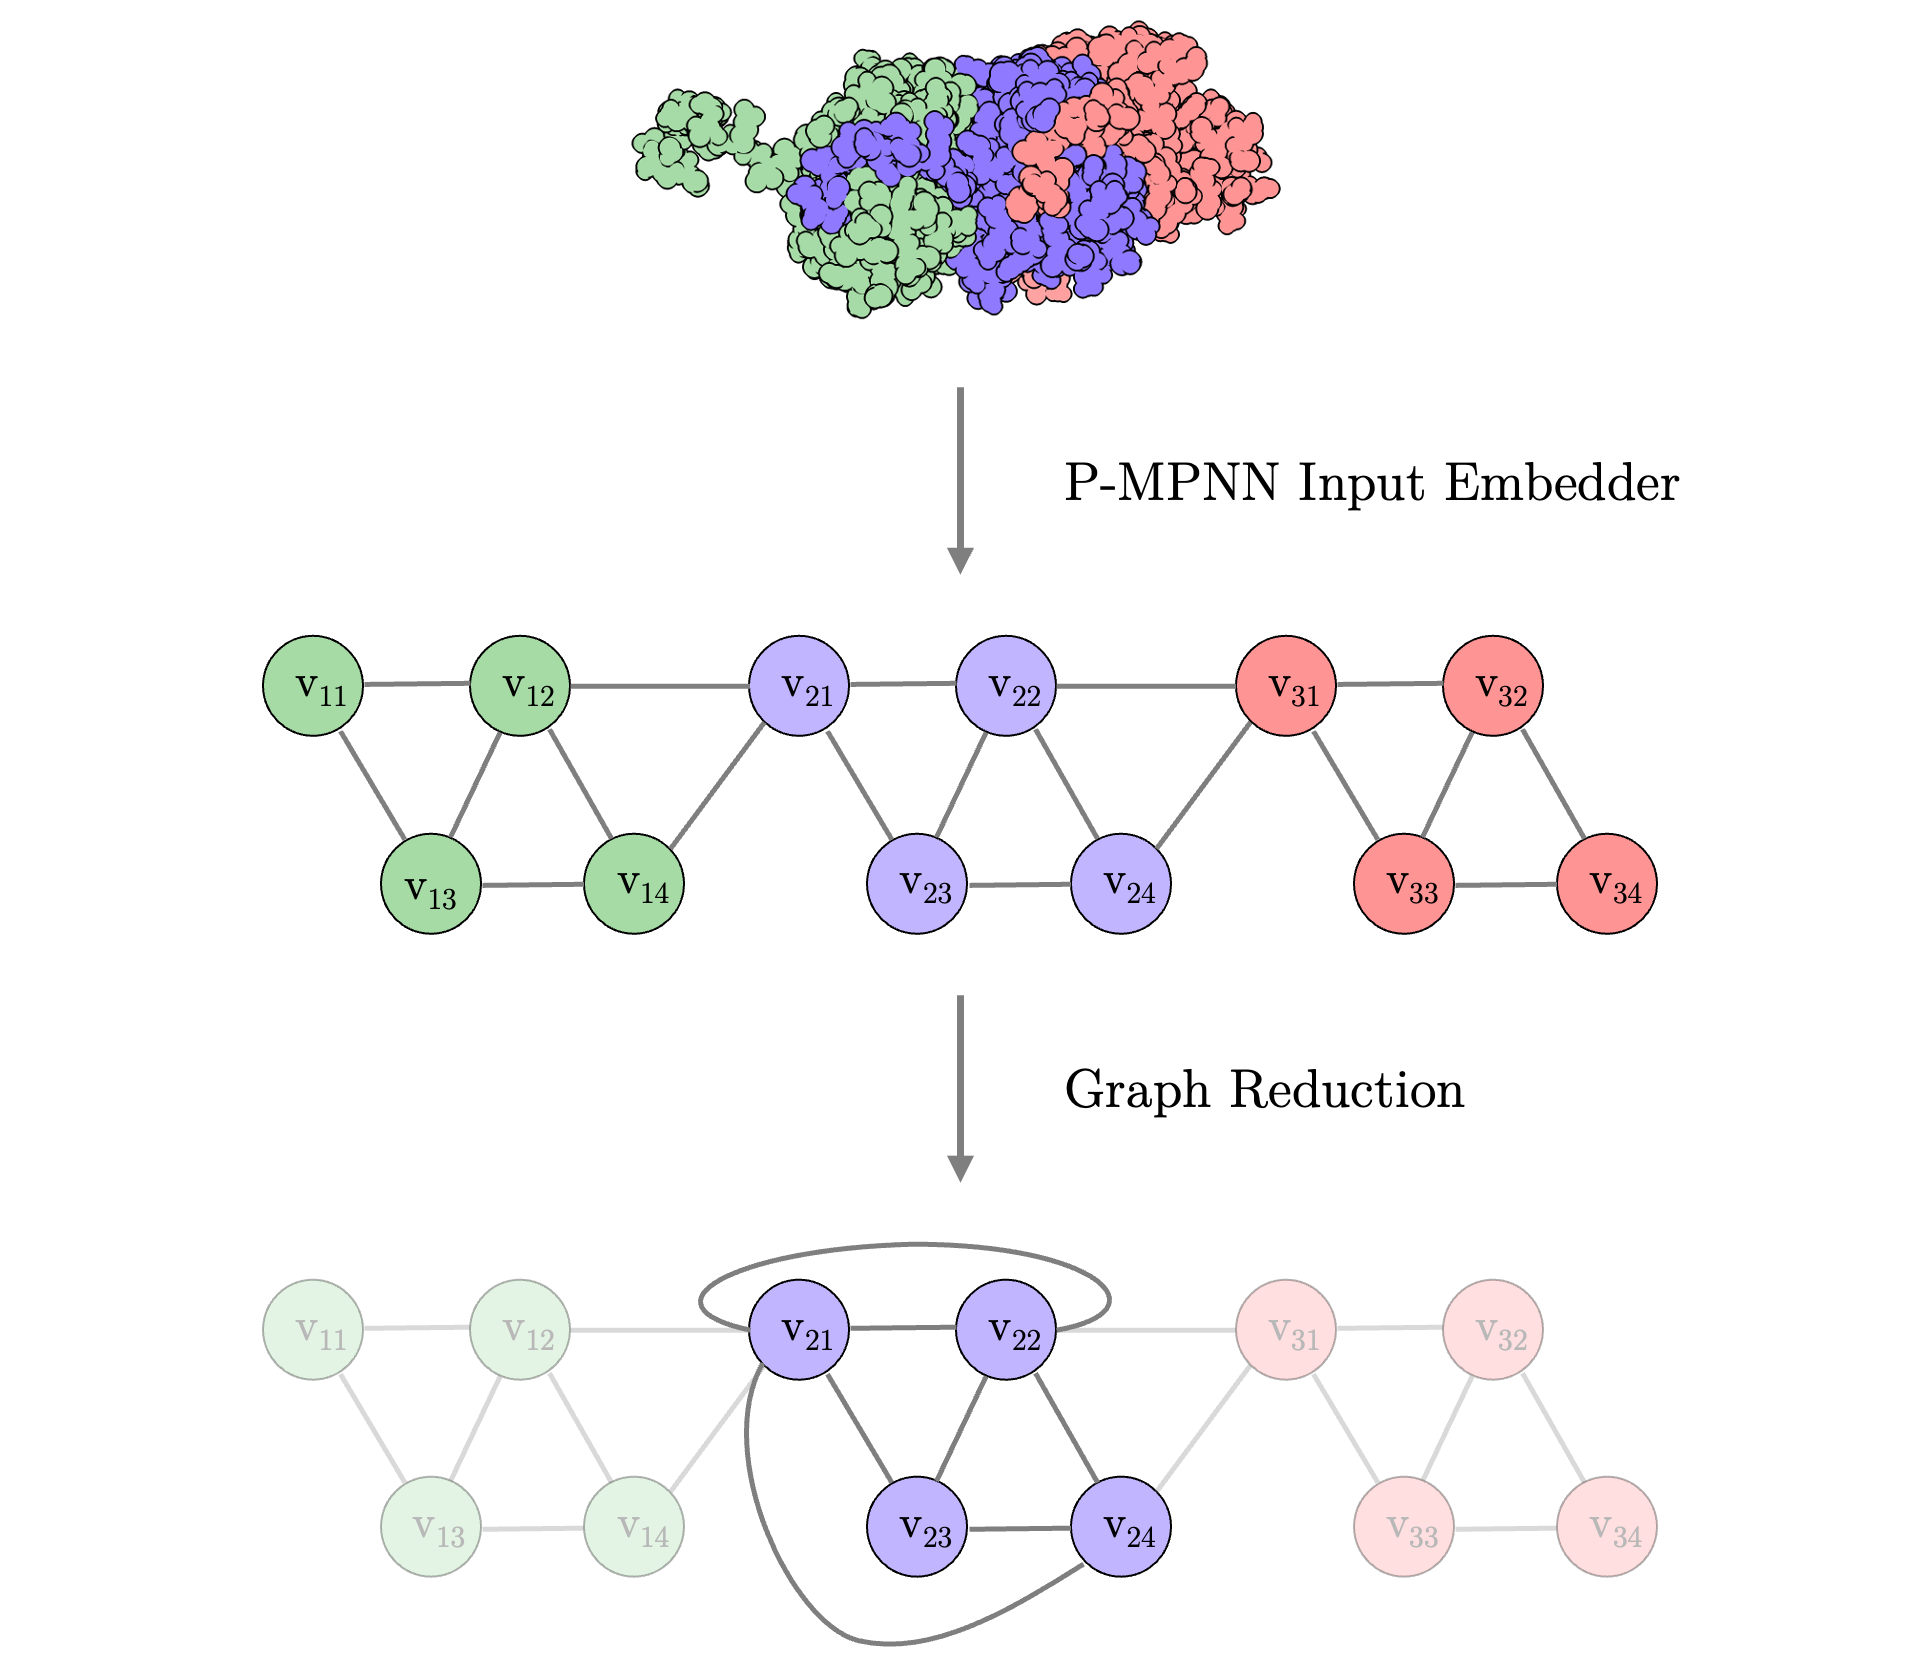
\includegraphics[width=\textwidth]{pmpnn_graph.png}
\caption{\textbf{Graph Reduction procedure for symmetric homooligomers.} After the default graph initialization from ProteinMPNN, one of the monomers is chosen as the reference monomer. Edges going out from it to other monomers are remapped to the corresponding residue in itself. Afterward, vertices and edges of the non-reference monomers are discarded. }
\label{fig:pmpnn_graph}
\end{figure}

When testing this new algorithm for different helical viruses, the Graph Reduction procedure showed no significant improvement compared to prediction based on a 2x2 neighborhood or a 3x3 neighborhood of monomers (\autoref{fig:pmpnn_comp}). For PVX and Tobacco Mosaic Virus (TMV), the three multimeric inputs (2x2 / 3x3 / infinite neighborhood) performed better than prediction based on a sole monomer, while no such improvement was observed for Pepino Mosaic Virus (PepMV) and Bamboo Mosaic Virus (BaMV) where all methods had similar sequency recovery rates. These results suggest that for the tested proteins, the incorrect neighborhood for small crops doesn't lead to an increased call of wrong amino acids in the aggregated logits. The newly developed infinite symmetry approach performs en par with 2x2 or 3x3 neighborhood prediction, but lowers the amount of required compute to that of a single monomer. However, it is to note that compute cost is generally not a concern when running ProteinMPNN due to its low complexity. 

\begin{figure}
\centering
\includesvg[width=\textwidth]{modeling/pmpnn_comparison.svg}
\caption{\textbf{Sequence recovery by ProteinMPNN for different input configurations.} The input was chosen as either a single monomer, a 2x2 neighborhood, a 3x3 neighborhood, or a symmetry-preserving graph reduction, modeling a theoretical infinite neighborhood. For each of the four targets Potato Virus X (PVX), Tobacco Mosaic Virus (TMV), Pepino Mosaic Virus (PepMV) and Bamboo Mosaic Virus (BaMV), each model was evaluated 50 times using random decoding orders and a sampling temperature $\tau\rightarrow 0$. The errorbars indicate the standard deviation over the repeated evaluation. }
\label{fig:pmpnn_comp}
\end{figure}

ProteinMPNN was used to generate sequences based on the wildtype backbone structure of PVX using the introduced Graph Reduction technique to model an infinite symmetry and a sampling temperature of $\tau\rightarrow 0$, e.g. argmax sampling. Sequences were generated with varying bias $b$ towards the wildtype sequence, that is by increasing the logit of the residue that's present in the wildtype structure by $b$ before sampling the amino acid. For each of the bias values $b \in \{0, 1, 2, 2.5\}$, five sequences. The sequence identity of the generated sequences to the wildtype was about $0.54$ (bias $0$), $0.73$ (bias $1$), $0.88$ (bias $2$) and $0.94$ (bias $2.5$). The generated sequences were further analyzed as described in the \autoref{ch:alphafold} and \autoref{ch:gromacs} before selecting some for experimental evaluation. 